% !TEX root = ../main.tex
%---------------------------------------------------------------------------------------------------
%---------------------------------------------------------------------------------------------------
\section{Modeling framework}\addtocounter{framenumber}{-1}
%---------------------------------------------------------------------------------------------------
%---------------------------------------------------------------------------------------------------
\begin{frame}\frametitle{Setup}\vspace{0.3cm}


  \heading{Structural econometric model}\vspace{-0.3cm}
  \begin{align*}
    \mathbb{R}^n \supset \bTheta \ni \btheta \mapsto  \M(\btheta) = y
  \end{align*}

  \pause
  \heading{Notation}
  \begin{columns}
  \begin{column}{0.5\textwidth}
    \begin{align*}\begin{array}{ll}
    \M & \text{mapping under status-quo} \\[0.5em]
    \M_g & \text{mapping under policy $g$}  \\[0.5em]
    \btheta_0 & \text{true parameter} \\[0.5em]
    \end{array}\end{align*}
  \end{column}
  \begin{column}{0.5\textwidth}
    \begin{align*}\begin{array}{ll}
    y_g         & \text{counterfactual} \\[0.5em]
    \hat{\btheta} & \text{estimated parameter} \\[0.5em]
    \bTheta(\alpha) & \text{confidence set with coverage $1 - \alpha$} \\[0.5em]
    \end{array}\end{align*}
  \end{column}
  \end{columns}

\end{frame}
%---------------------------------------------------------------------------------------------------
%---------------------------------------------------------------------------------------------------
\begin{frame}{Comparing models}
  \begin{figure}[h!]\centering
  \scalebox{0.3}{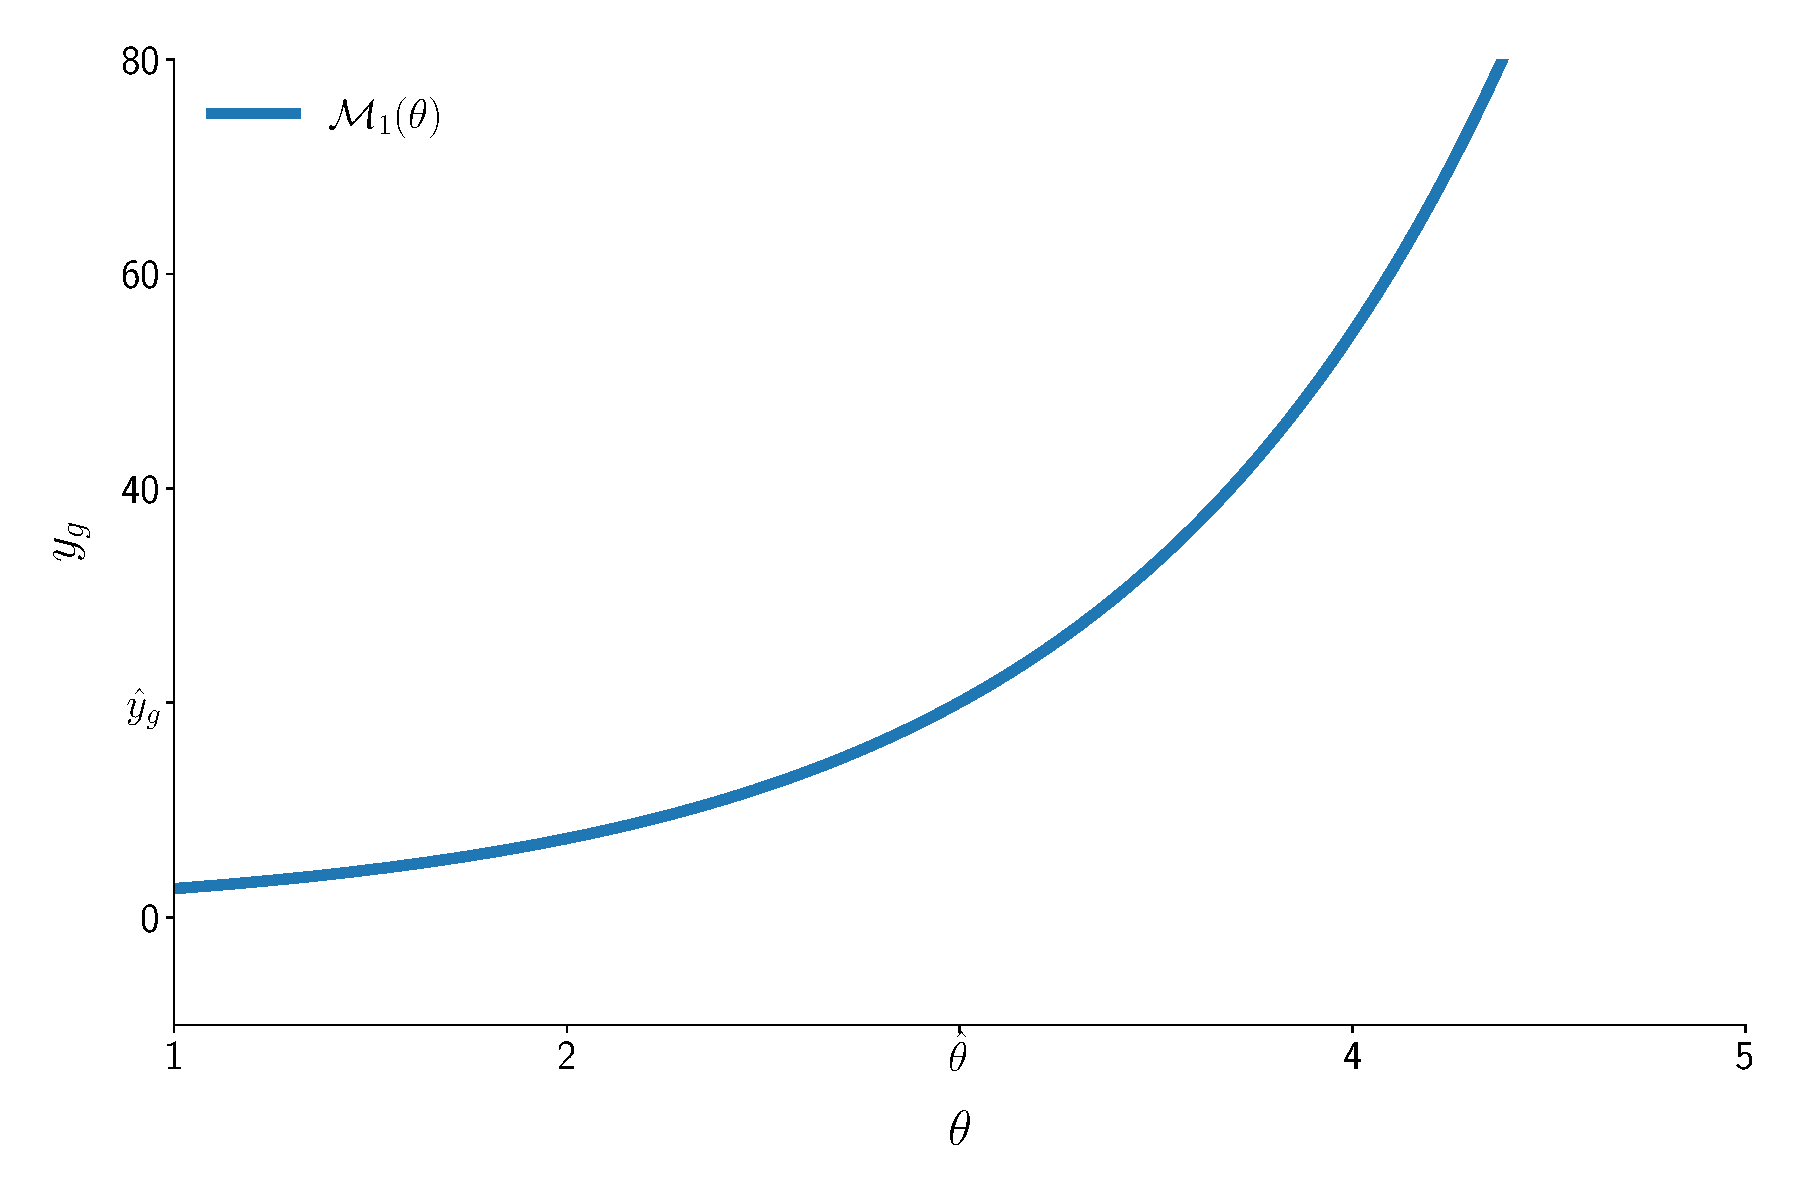
\includegraphics{fig-illustration-comparison-model-1.pdf}}
  \end{figure}
\end{frame}\addtocounter{framenumber}{-1}
%---------------------------------------------------------------------------------------------------
%---------------------------------------------------------------------------------------------------
\begin{frame}{Comparing models}
  \begin{figure}[h!]\centering
  \scalebox{0.3}{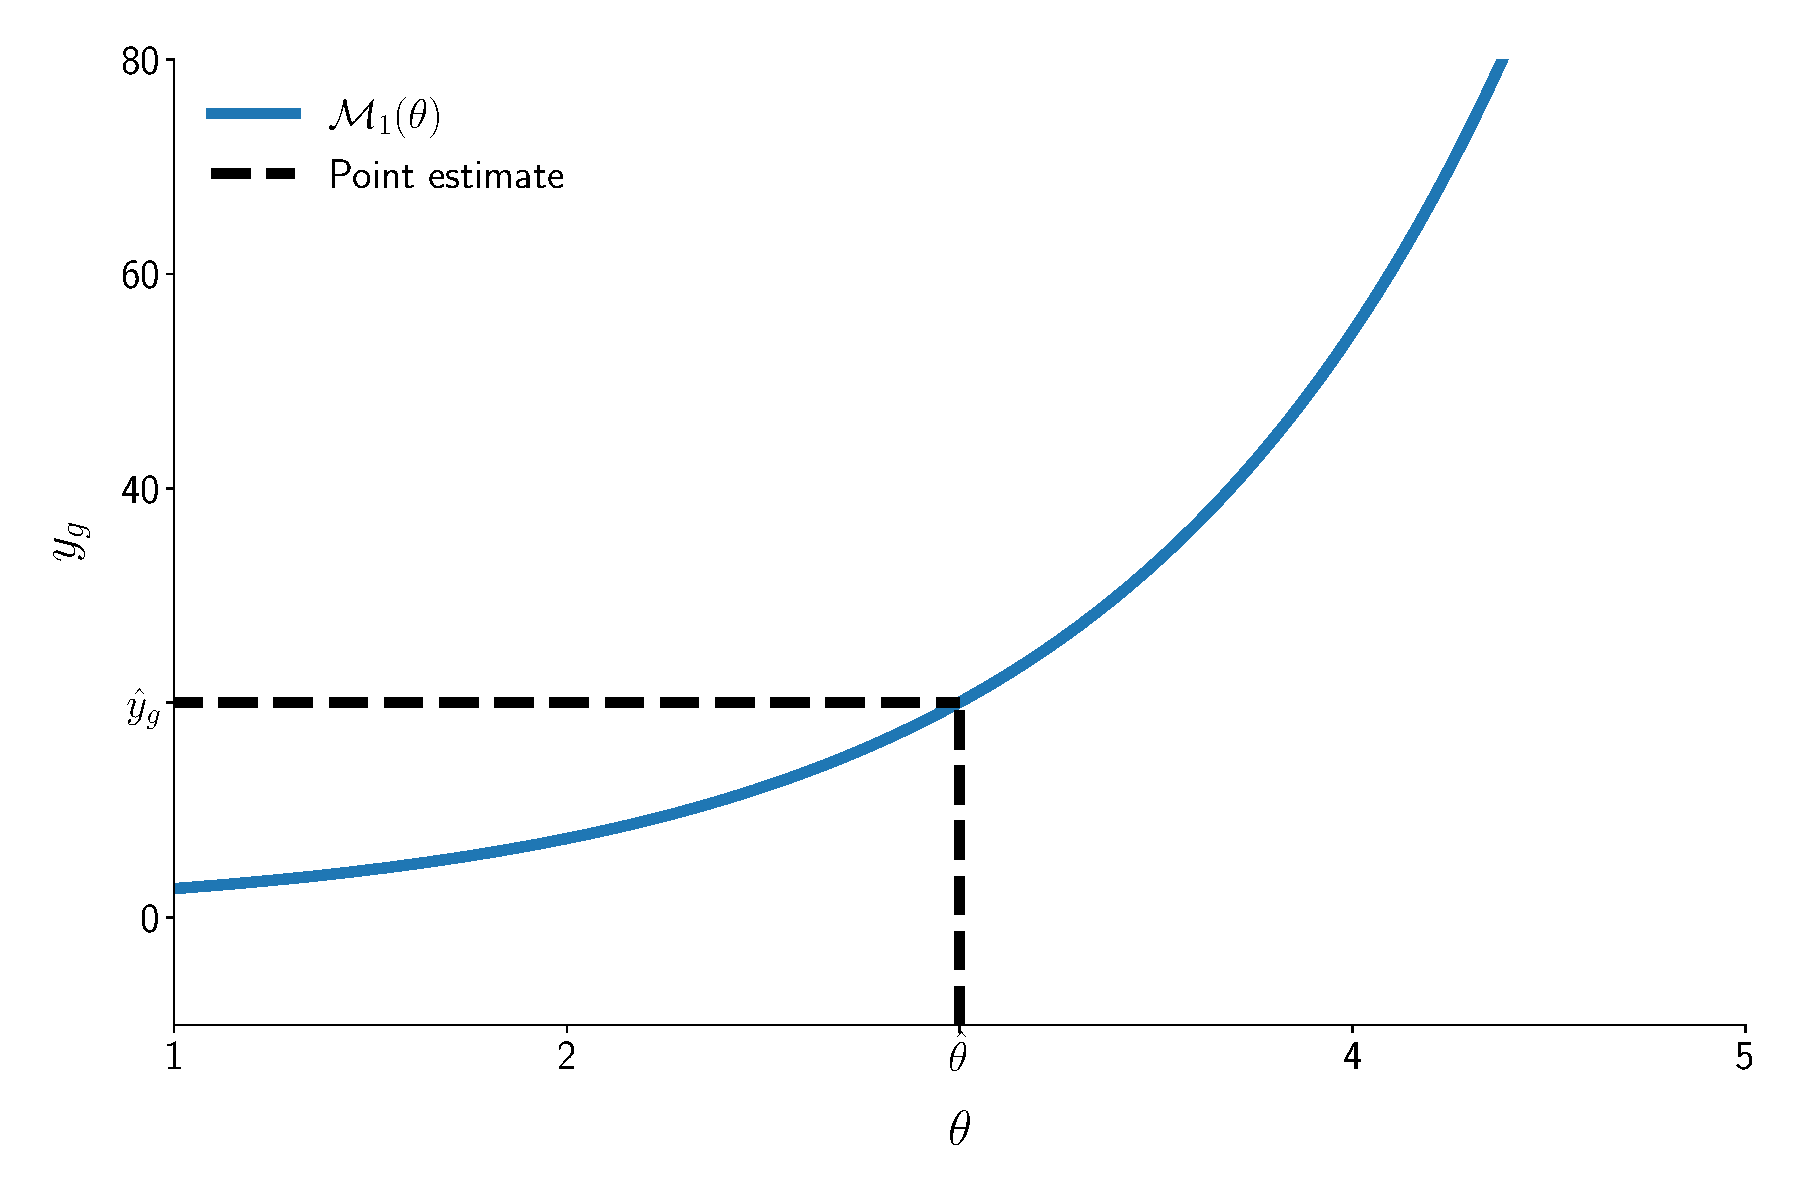
\includegraphics{fig-illustration-comparison-model-2.pdf}}
  \end{figure}
\end{frame}\addtocounter{framenumber}{-1}
%---------------------------------------------------------------------------------------------------
%---------------------------------------------------------------------------------------------------
\begin{frame}{Comparing models}
  \begin{figure}[h!]\centering
  \scalebox{0.3}{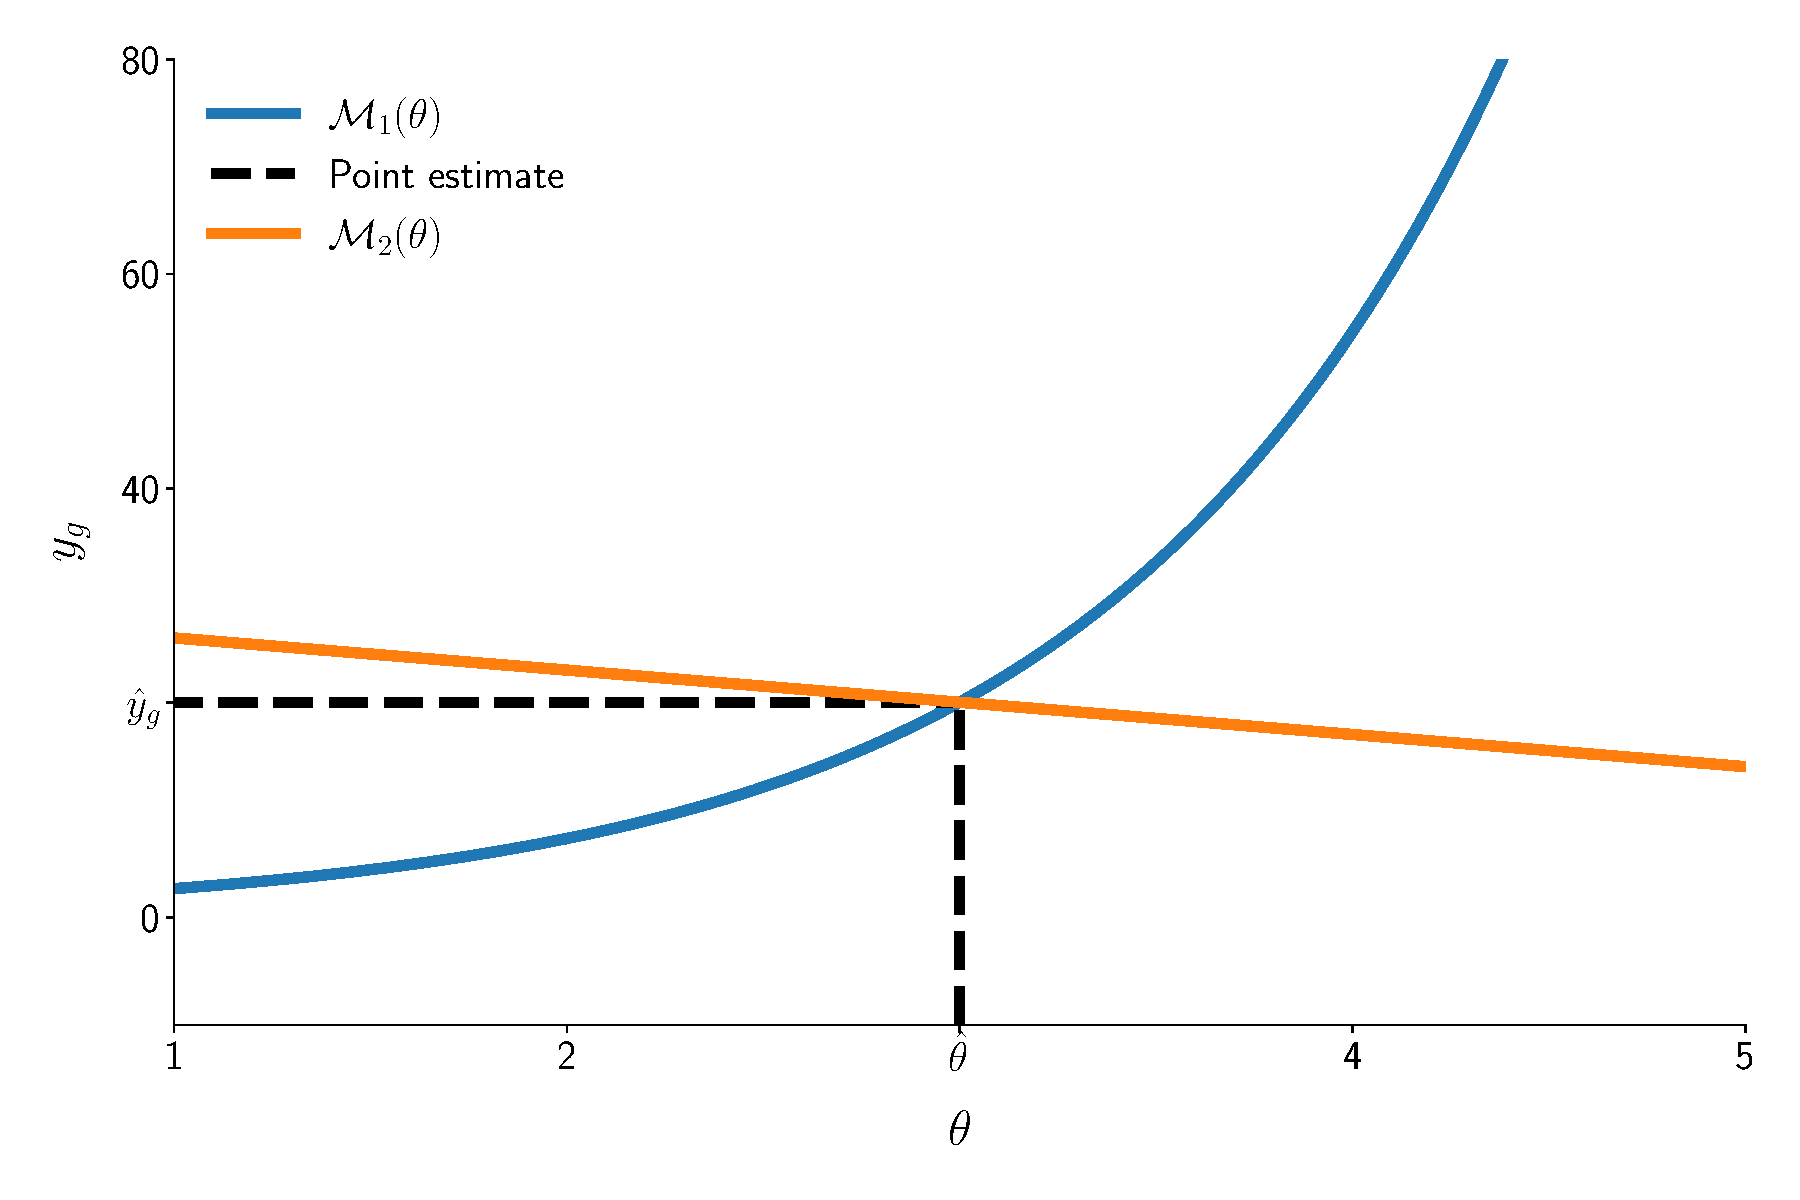
\includegraphics{fig-illustration-comparison-model-3.pdf}}
  \end{figure}
\end{frame}\addtocounter{framenumber}{-1}
%---------------------------------------------------------------------------------------------------
%---------------------------------------------------------------------------------------------------
\begin{frame}{Comparing models}
  \begin{figure}[h!]\centering
  \scalebox{0.3}{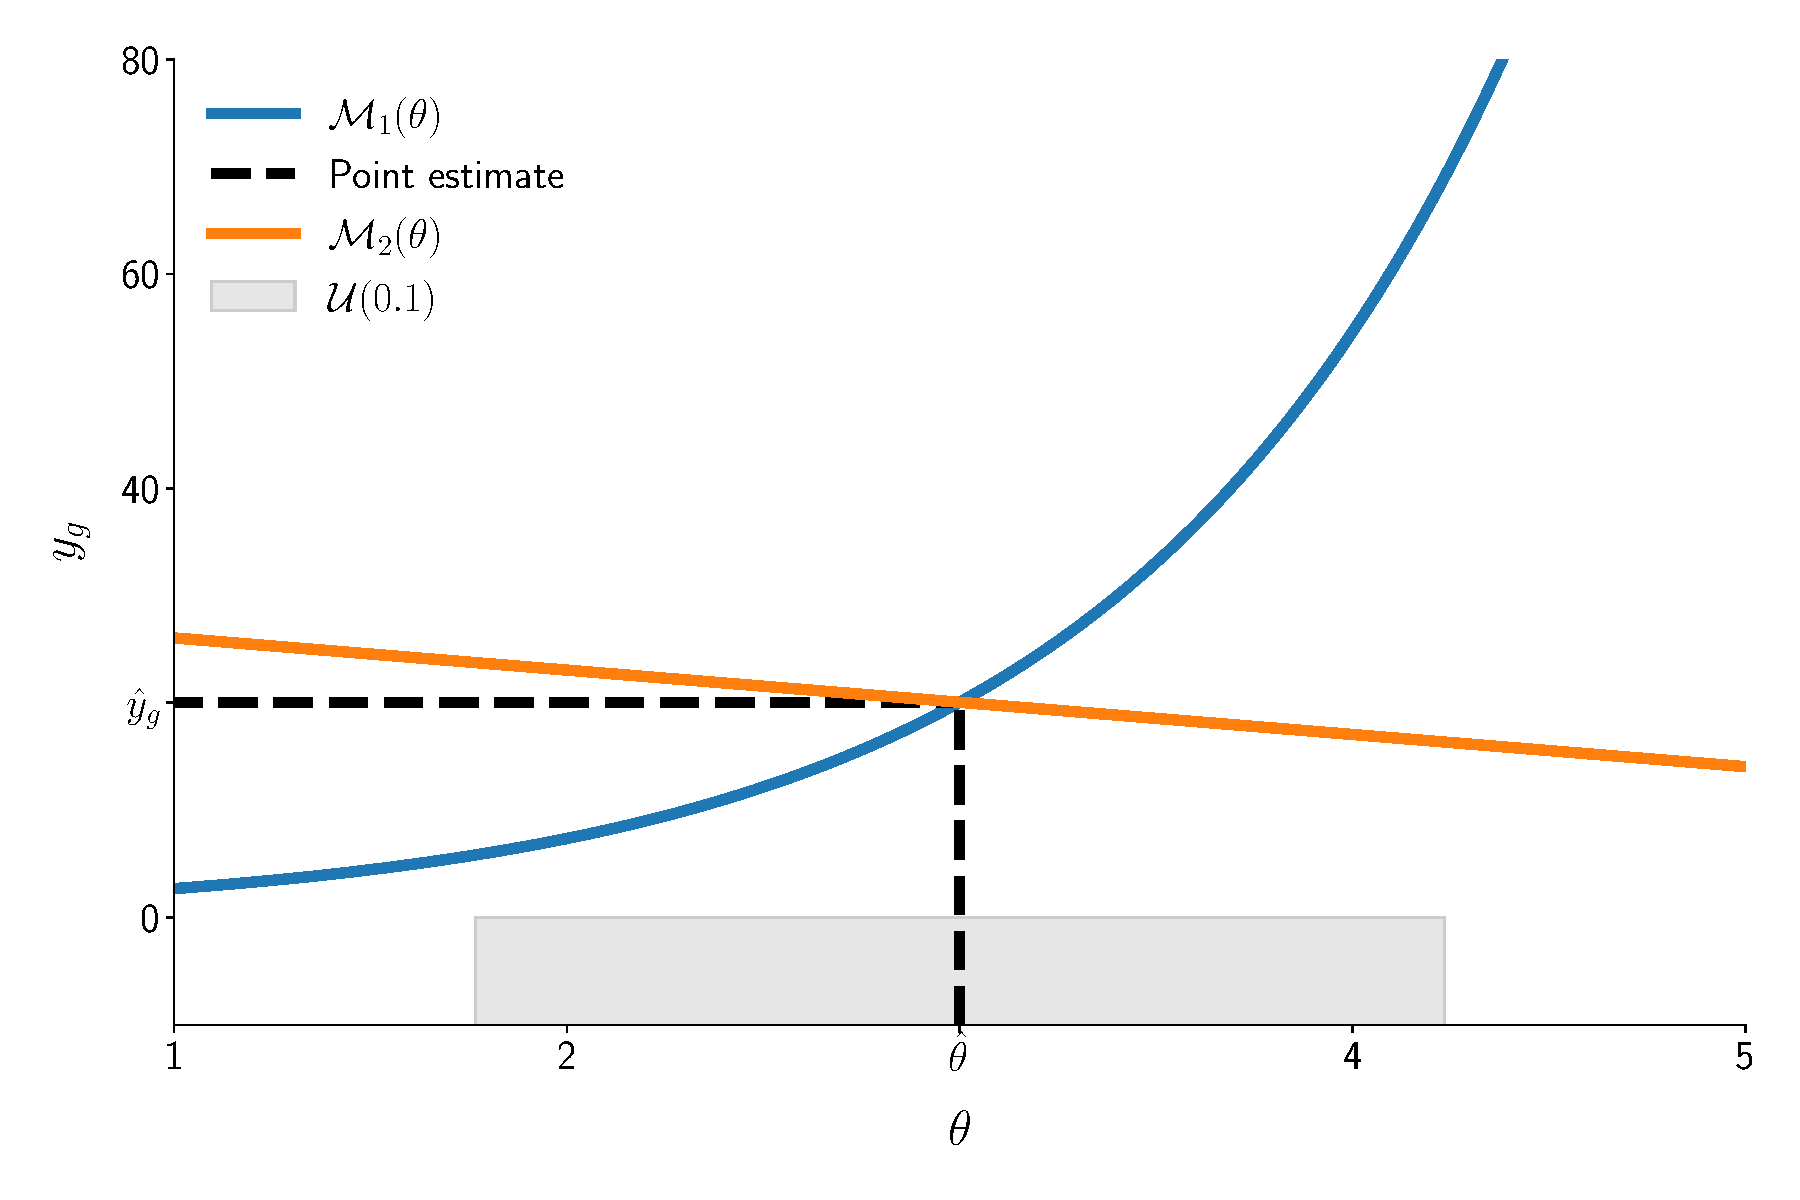
\includegraphics{fig-illustration-comparison-model-4.pdf}}
  \end{figure}
\end{frame}\addtocounter{framenumber}{-1}
%---------------------------------------------------------------------------------------------------
%---------------------------------------------------------------------------------------------------
\begin{frame}{Decision-theoretic framework}\vspace{0.25cm}


\heading{As-if decisions with point estimates}\vspace{0.3cm}
\begin{itemize}
  \item \only<1-6>{\makebox[0pt][l]{As-if optimization}\phantom{spacespacespacespace}} \only<2-6>{$\quad g^* =\argmax_{g \in \G} M_g({\color{red} \hat{\btheta}})$}
\end{itemize}\vspace{0.4cm}

\pause\pause

\heading{As-if decisions with set estimates \citep{Manski.2021}}\vspace{0.3cm}
\begin{itemize}
  \item \only<3-6>{\makebox[0pt][l]{Maximin criterion}\phantom{spacespacespacespace}} \only<4-6>{$\quad g^* =\argmax_{g \in \G} \min_{\btheta \in {\color{red} \U(\alpha)}} M_g(\btheta)$}

  \item[]
  \item \only<3-6>{\makebox[0pt][l]{Minimax regret rule}\phantom{spacespacespacespace}} \only<5-6>{$\quad g^* =\argmin_{g \in \G} \max_{\btheta \in {\color{red}\U(\alpha)}} \left[\max_{\tilde{g} \in \G} M_{\tilde{g}}(\btheta) - M_g(\btheta) \right]$}

  \item[]
  \item \only<3-6>{\makebox[0pt][l]{Subjective Bayes}\phantom{spacespacespacespace}} \only<6>{$\quad g^* =\argmax_{g \in \G} \int_{ {\color{red} \U(\alpha)}} M_g({\btheta}) \dd{f(\btheta)}$}

\end{itemize}

\end{frame}
%---------------------------------------------------------------------------------------------------
%---------------------------------------------------------------------------------------------------
\begin{frame}{Comparing policies}
  \begin{figure}[h!]\centering
  \scalebox{0.3}{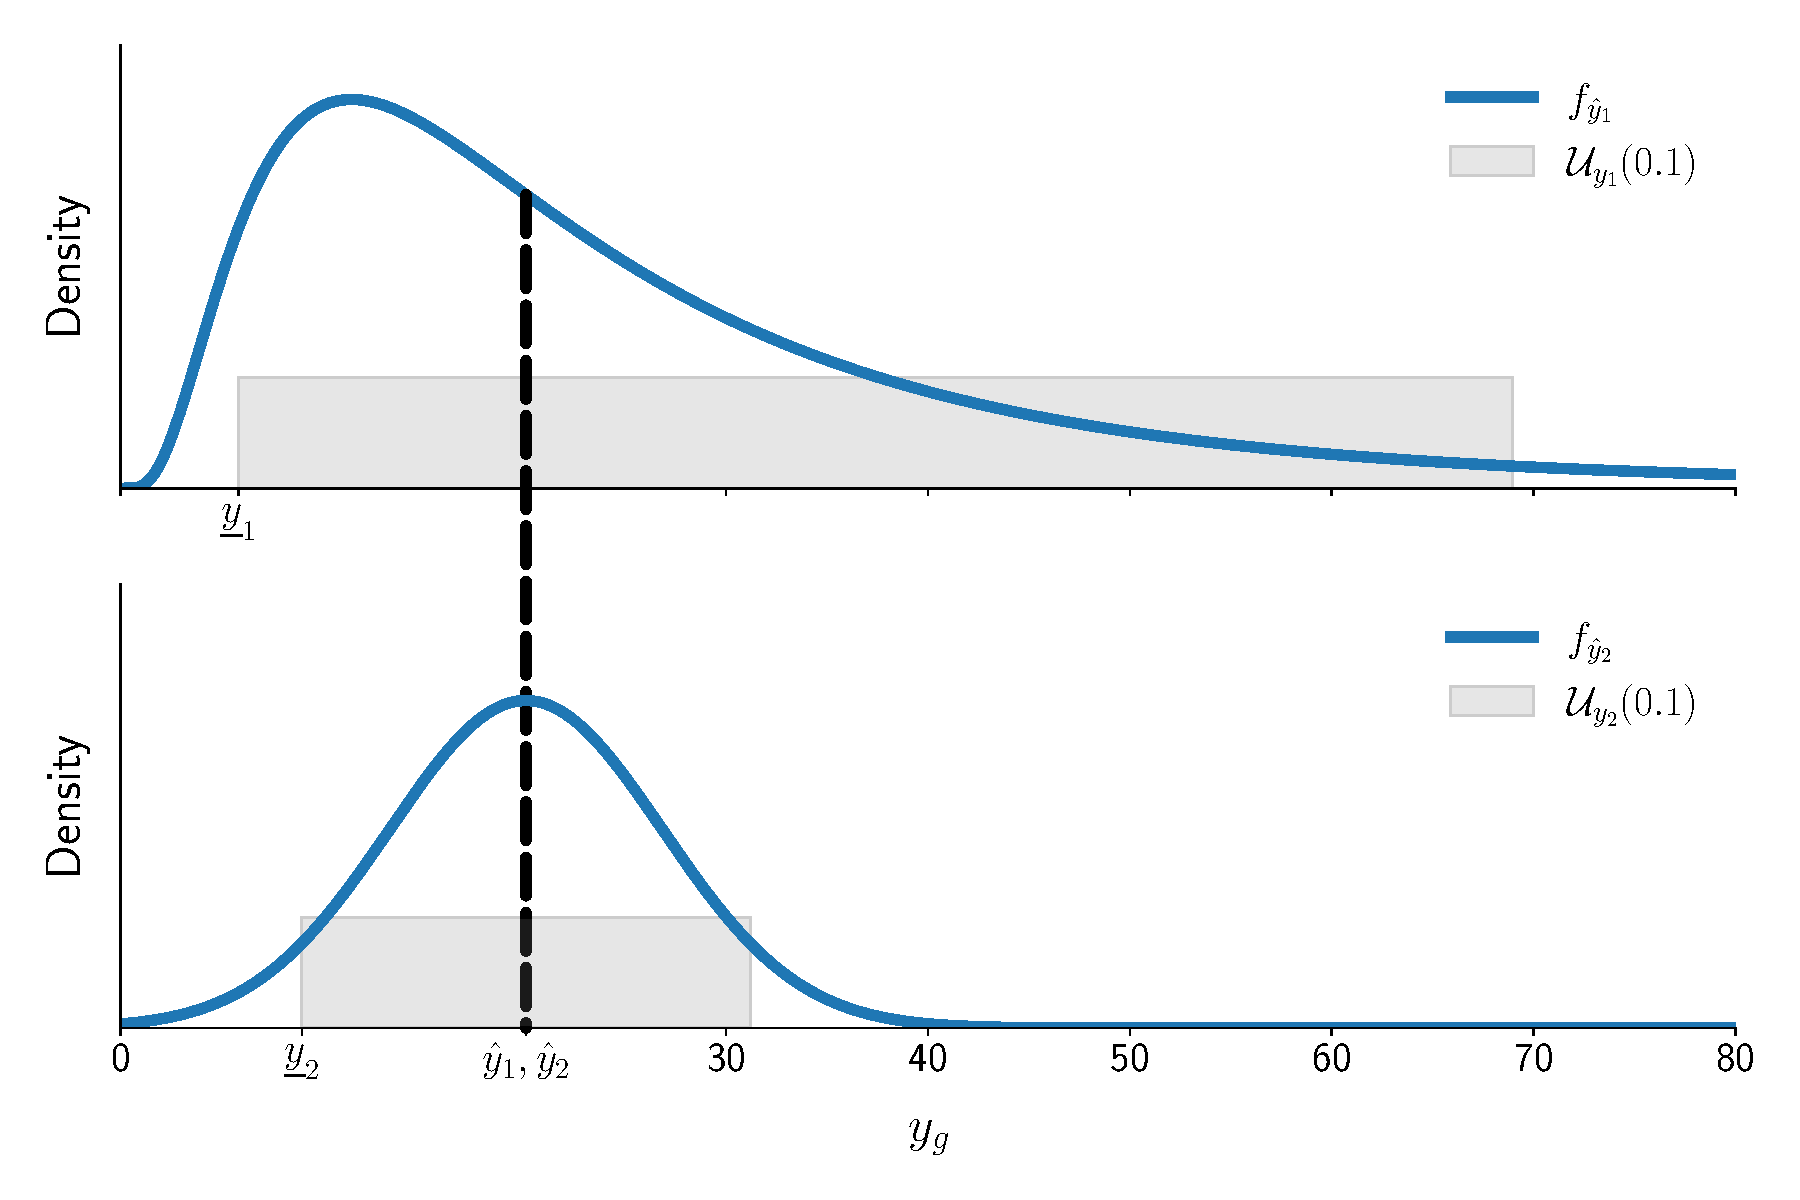
\includegraphics{fig-illustration-comparison.pdf}}
  \end{figure}
\end{frame}
%---------------------------------------------------------------------------------------------------
%---------------------------------------------------------------------------------------------------
\begin{frame}{Comparing policies}
  \begin{figure}[h!]\centering
  \scalebox{0.3}{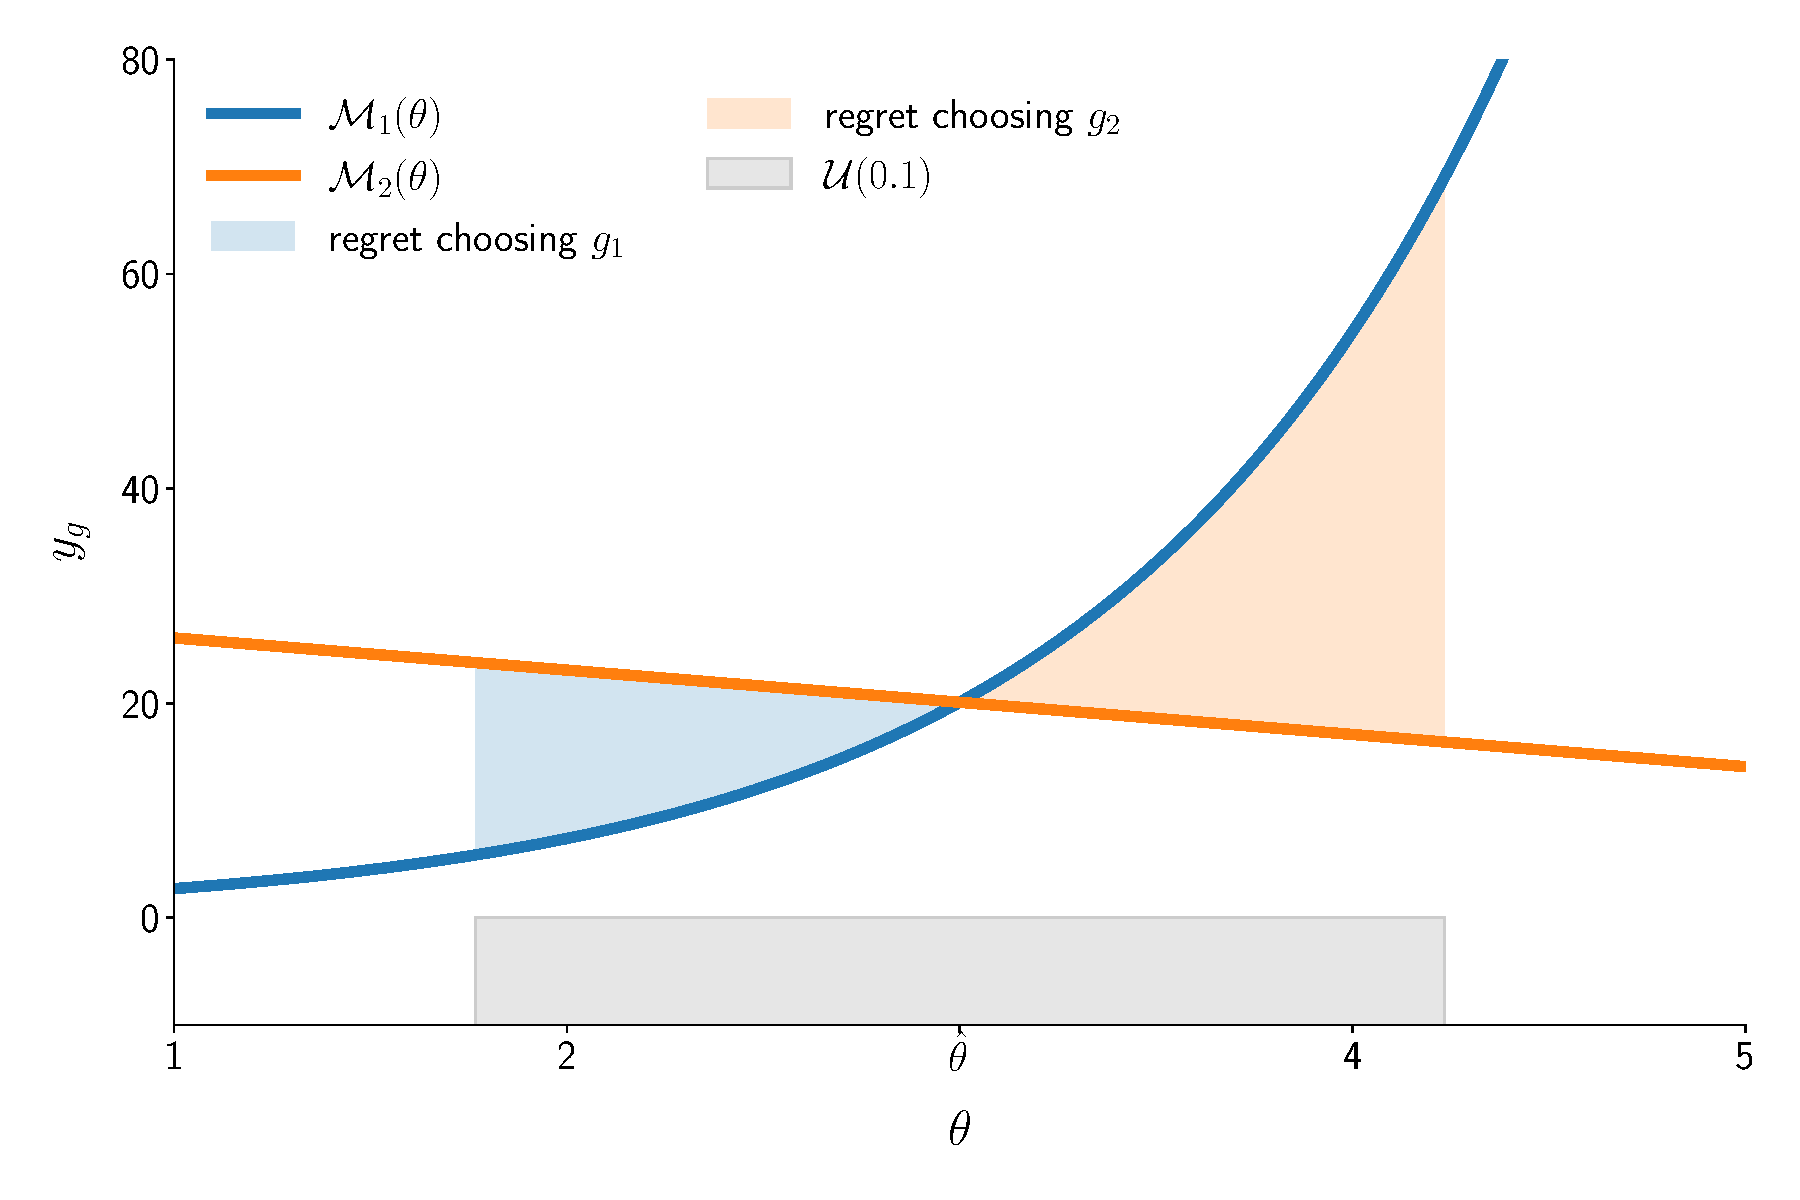
\includegraphics{fig-illustration-comparison-regret.pdf}}
  \end{figure}
\end{frame}
%---------------------------------------------------------------------------------------------------
%---------------------------------------------------------------------------------------------------
\begin{frame}{Comparing policies}
  \begin{figure}[h!]\centering
  \scalebox{0.3}{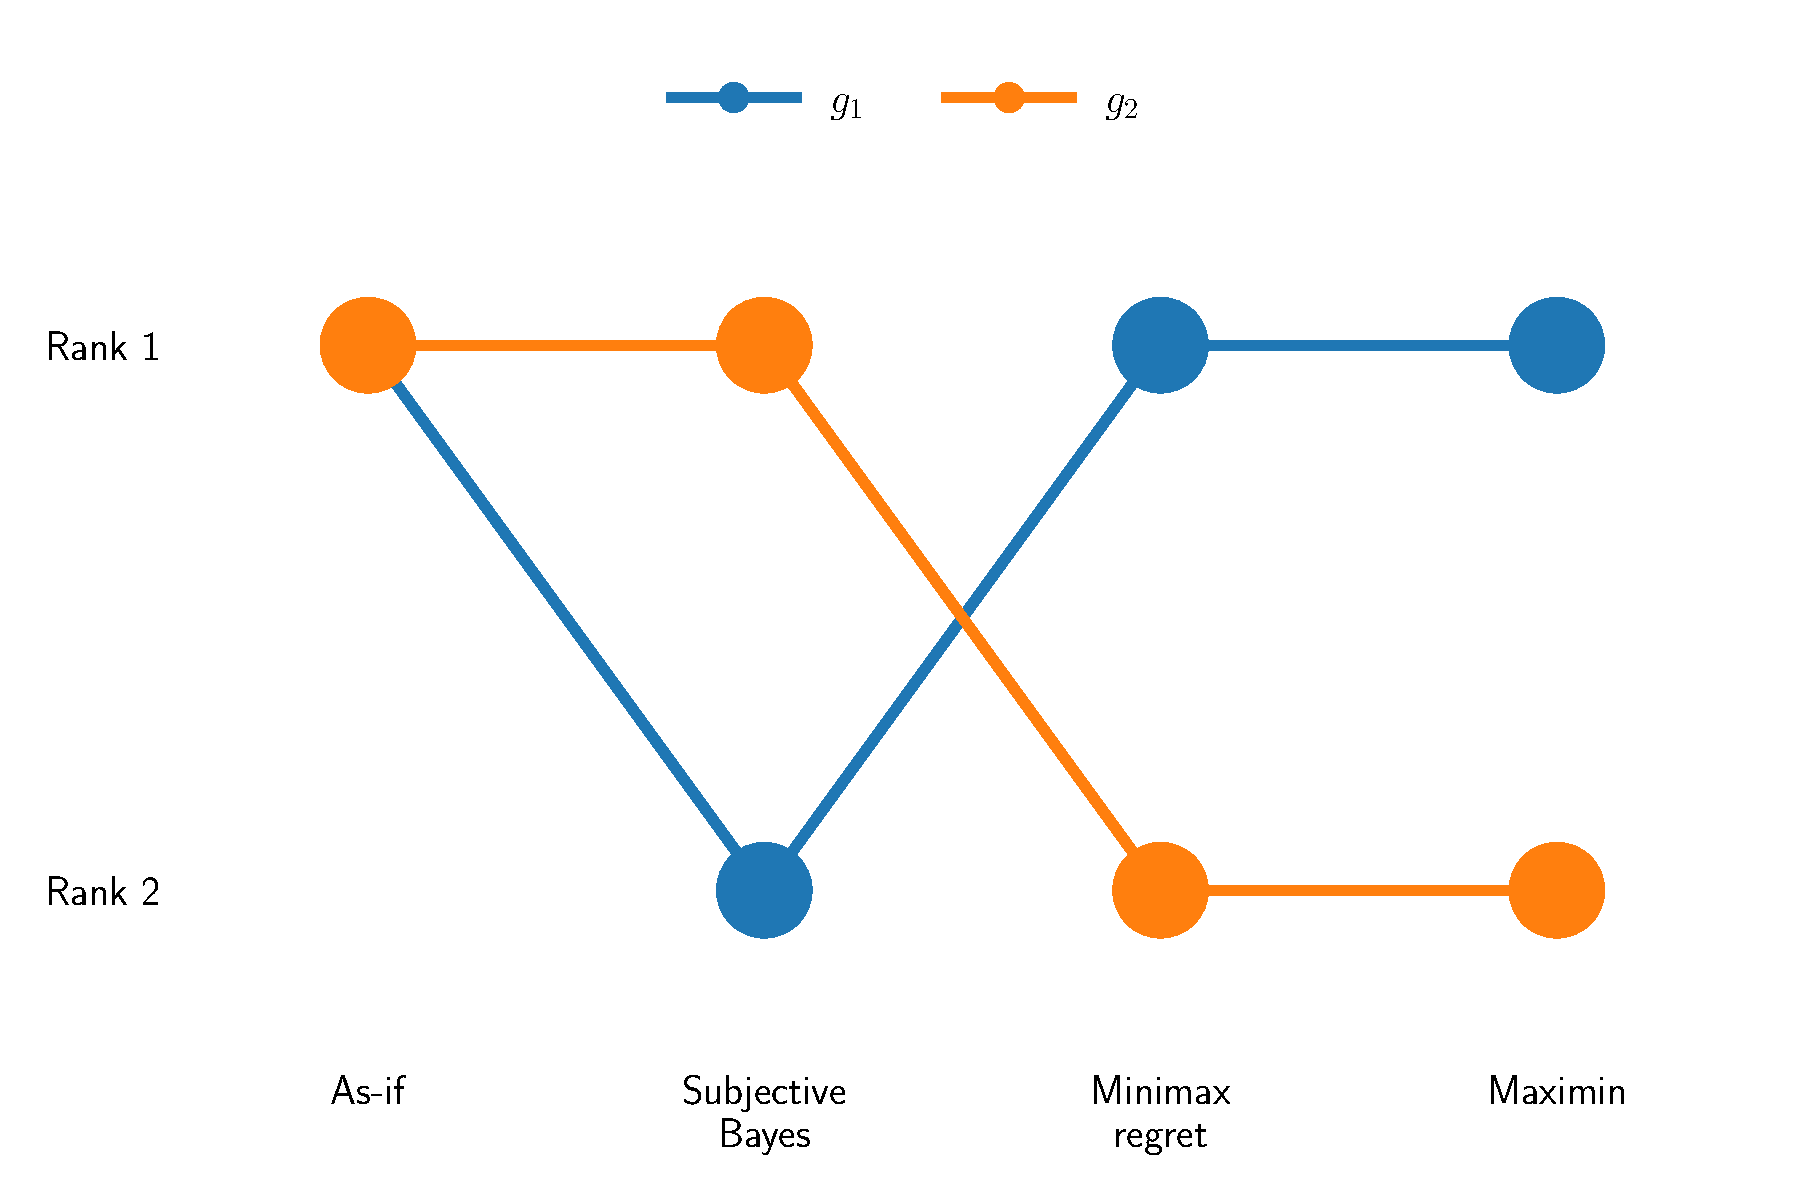
\includegraphics{fig-illustration-criterion-policy-ranks.pdf}}
  \end{figure}
\end{frame}
%---------------------------------------------------------------------------------------------------
%---------------------------------------------------------------------------------------------------
